\documentclass[conference]{IEEEtran}
\IEEEoverridecommandlockouts
% The preceding line is only needed to identify funding in the first footnote. If that is unneeded, please comment it out.
\usepackage{cite}
\usepackage{amsmath,amssymb,amsfonts}
\usepackage{cite}
\usepackage{algpseudocode}
\usepackage{graphicx}
\usepackage{textcomp}
\usepackage{xcolor}
\usepackage{amsthm}
\usepackage{algorithm}
%\usepackage{algorithmic}
\usepackage{epstopdf}
\usepackage{subfigure}
\usepackage{verbatim}
\usepackage{diagbox}



\newcommand{\tabincell}[2]{\begin{tabular}{@{}#1@{}}#2\end{tabular}}
\def\BibTeX{{\rm B\kern-.05em{\sc i\kern-.025em b}\kern-.08em
    T\kern-.1667em\lower.7ex\hbox{E}\kern-.125emX}}
\begin{document}

\title{Workload-Aware Scheduling for Heterogeneous Storage Data Analytics\\
}

\author{\IEEEauthorblockN{name1, name2, name3, and name4}
\IEEEauthorblockA{State Key Lab. for Novel Software Technology, Nanjing University, CN\\
Email: email address, \{email address\}@nju.edu.cn}}


\maketitle

\begin{abstract}
A trend in nowadays data centers is that equipped with SSD, HDD, etc., heterogeneous storage devices are widely deployed to meet different demands of various big data workloads. Since the read speeds of diverse storage devices are quite different, the unbalanced use on either specific type of storage or particular device would easily overload them, making them being hotspots and finally worsen the read performance for analytical tasks. In this paper, we formulate Workload-Aware Scheduling problem for Heterogeneous Storage (WASH), and show its NP-hardness. To solve this problem, we propose a randomized algorithm (WASH-rdm) which can be proved concentrated on its optimum value with high probability through our theoretical analysis. Our extensive Experiments show that the WASH-rdm can reduce the task reading time by up to 55\% over the state-of-the-art baseline algorithm.
%In order to meet different storage requirements, various heterogeneous storage hardware, such as SSD, HDD and so on, are widely deployed in data centers. Due to different production standards and different usage frequencies, these heterogeneous storage hardware usually have great differences in read performance. Traditional scheduling mechanism usually neglect the hardware where data is stored. On the one hand, it is likely that a large number of tasks choose low-performance disks to read data. On the other hand, it is possible for task to choose overloaded disks to read data. Therefore, the traditional method may lead to the task reading process becoming bottleneck. In this paper, we formulate the above problem as Workload-Aware Scheduling for Heterogeneous Storage problem (WASH), and show its NP-hardness. To solve this problem, we propose a heuristic algorithm (WASH-greedy) and a guaranteed performance random algorithm (WASH-rdm). WASH-rdm can be proved concentrated around its optimum value with high probability. Experiments show that the our algorithm can reduce the task reading time by up to 55\% over the state-of-the-art baseline algorithm.

%such as large capacity, high-speed and so on, 
%Nowadays, a trend in data center is that there are more and more heterogeneous storage devices, i.e. SSD and HDD, which may differ greatly in performance. However, data processing frameworks such as MapReduce often considers that hardware is homogeneous and task scheduling is not aware of the difference between heterogeneous storage devices. In this case, if a large number of tasks are scheduled on low-speed storage nodes, it will greatly cause data processing bottlenecks. Furthermore, due to the different performance of each disk, it is difficult to make all disks have the balanced load. In this paper, we formulate the above problem as Heterogeneous Storage-aware Task Scheduling Problem (HTS), and show its NP-hardness. In order to solve this problem, we propose a heuristic algorithm and a random algorithm whose distance from the optimum value is within $t$ with high probability. Experiments show that the our algorithm can reduce the task execution by up to 55\% over the storage-unaware scheduling mechanism.
\end{abstract}

\begin{IEEEkeywords}
big data analytics, heterogeneous storage, workload-aware scheduling
\end{IEEEkeywords}

\section{Introduction}

Nowadays, there are new trend that data centers have a variety of workloads, e.g., some data analytical applications and other machine learning based applications like Grep and K-NN \cite{b27}. The different workloads might have different requirements on storage performance \cite{b28} \cite{b29} \cite{b30} \cite{b31}. For example, K-NN is compute-intensive application whose execution time accounts for a large proportion while Grep is I/O-intensive application which has a great throughput. In order to meet these demands, big data processing platforms, e.g., Hadoop\cite{b14} and Spark\cite{b15}, have deployed a lot of heterogeneous devices.

However, the heterogeneity of these devices would lead to the divergent read performances which lies in two aspects. Firstly, the different types of storage, e.g. SSD \cite{b32} and HDD\cite{b33}, have different read performances. For example, as shown in Fig.\ref{Fig:motivation} reading the same amount of data from HDD takes almost twice longer than SSD. Secondly, when there are a large number of tasks reading from specific device, it will also lead to poor read performance. As shown in Fig.\ref{Fig:motivation}, when the amount of tasks increases, the time required for each task will also increase.

Due to the different read performances, traditional scheduling may result in unbalanced usage on storage device. For example, when tasks fetch data from those disks with higher read performance, they would spend less on time I/O, compared with those with lower read performance disk. Furthermore, the data analytical tasks which are deployed on them will be enlarged. As a result, disks with poor read performances or heavy workload would elongate the I/O performance of analytical tasks.

%For example, when the same number of read tasks are deployed on disks with different read performances, low-performance disks may have read hotspots.
%Nowadays, in data centers that support big data processing platforms, i.e., Hadoop\cite{b14} and Spark\cite{b15}, there are more and more heterogeneous devices. On the one hand, due to the purchase of hardware devices from different hardware providers, such as Seagate\cite{b16} and Samsung\cite{b17}, the different standard hardware lead to heterogeneous; on the other hand, the use and maintenance of equipment may also lead to heterogeneous. However, the underlying heterogeneity of storage is often neglected in general scheduling mechanism, which always results in disk bottleneck. Furthermore, it affects the completion time of tasks and the result is the low performance of big data analytics.
%which results in the mismatch between upper software and lower hardware.
\begin{figure}[!t]
	\centering
	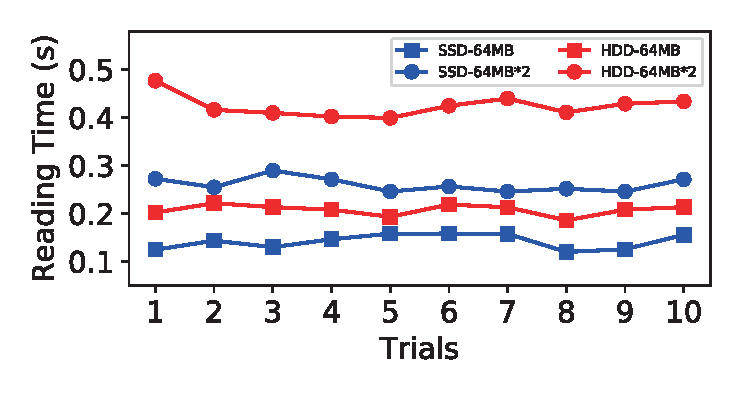
\includegraphics[height=1.8in]{fig_motivation5.eps}
	\caption{Comparisons of 1) the time required for one task to read 64MB, 2) the time required for two tasks to read 64MB at the same time, i.e., 128MB, from heterogeneous storage SSD and HDD, for 10 times. Reading the same amount of data from HDD takes almost twice longer than SSD.}
	\label{Fig:motivation}
\end{figure} 

%However, due to the divergent read performance of different storage and the cumulative workload of the storage, its hard to hard to achieve this aim. 
 
Thus, we propose to focus on balanced usage of heterogeneous storage resources in this paper. However, due to the multiple replicas of data, how to choose these feasible location is a big challenge.
 Most of the research focuses on heterogeneous computing resources \cite{b25}\cite{b26}\cite{b35}\cite{b36}, ignoring the heterogeneous storage resources. Although some works considers heterogeneous storage \cite{b6}\cite{b7}, multiple storage types are not considered. In contrast, we formulate the Workload-Aware Scheduling problem and prove its NP-hardness. Then, we propose a randomized algorithm (WASH-rdm) with performance guaranteed to solve the problem.
%We focus on two aspects. One is the read performance of the disk itself, the other is the load of the disk, that is, the number of tasks that are reading the data from the disk. Focus on the above two points, we formulate it as an optimization problem and propose a heuristic algorithm (WASH-greedy) and a random algorithm (WASH-rdm) with guaranteed performance to solve the problem. %Experiments show that the performance of the proposed algorithm is 55\% better than the Storage-unaware scheduling mechanism. 
More concretely, our contributions are as follows: 

\begin{itemize}
%\item We present the necessity of sloving this problem by showing impact of reading data phase during the task execution.
\item To balance the workload on heterogeneous storage device, we propose workload-aware scheduling problem which is proved to be NP-hard. 
\item We propose randomized algorithm with performance-guaranteed to solve this problem. The WASH-rdm algorithm can be proved concentrated around its optimum value with high probability 1 - O($e^{-t^2}$) where $t$ is the concentration bound.
\item The results of our simulation show that the performance of the WASH-rdm algorithm improves by 55\% over the art-of-the-state algorithms.
%compared with the storage-unaware scheduling mechanism and by 20\% 
\end{itemize}

The rest of the paper is organized as follows. In Section \ref{RELATED_WORKS}, we present the related works of the HTS problem. Then we propose our system model and our algorithm in Section  \ref{SYSTEM_MODEL} and Section  \ref{DESIGN_ALGORITHM}. At last, we conclude this paper in Section \ref{CONCLUSION} by summarizing our main contributions.


\section{RELATED WORKS}\label{RELATED_WORKS}
The related works consist of two parts. For the first part, due to limited link bandwidth, some work is focused on data locality. Furthermore, in heterogeneous environments, it is not enough to consider data locality alone and some other studies have been carried out to accelerate data processing by studying hardware heterogeneity \cite{b1}.

Due to the limited network bandwidth resources in data center, if a large amount of data is transmitted between nodes during task execution, it will greatly affect the task performance. Therefore, processing data locally as much as possible can improve performance, e.g., placeing map task to the node which stores the input data. Matei et al. \cite{b2} proposes delay scheduling to assure data locality. Delay scheduling considers that when a node has idle slots, priority should be given to scheduling tasks with input data at that node, and delayed scheduling tasks without input data at that nodes. Ganesh \cite{b3} makes multiple replicas of high-frequency data by analyzing the access frequency of data, improve the data locality in this way. Cristina \cite{b4} proposes a distributed adaptive data replication algorithm DARE, which can help scheduler achieve better data locality. Jalaparti \cite{b5} believes that most of the production work is repetitive and predictable, which enables us to plan ahead. Coordinating and improving the tasks and data placement of these jobs can effectively reduce bandwidth usage and improve data locality. All of these work improves the performance of data processing by improving data locality.

However, in heterogeneous data centers, due to the different performance of data storage devices, task completion time is often different. At present, some of the existing work is based on the research of storage heterogeneity, which accelerates the speed of data processing. Xu et \cite{b6} considers the current usability of underlying hardware (CPU, memory, I/O), but does not consider the performance differences of different storage hardware. 
In Hadoop 2.8, HDFS\cite{b19} considers heterogeneous storage and supports multiple storage strategies. One of the storage strategies is ONE\_SSD, that is, one replicas is stored in SSD, and the rest is stored in HDD. However, the task scheduling strategy is not aware of the disk's performance.
Based on ONE\_SSD, Pan \cite{b7} proposes H-Scheduler which takes into account the performance between HDD and SSD. Facing the trend of increasing heterogeneous storage, it is one-sided to divide the storage devices into two categories. Wang B \cite{b8} uses Markov model to describe the use of nodes in the cluster to deploy data reasonably. However, the scheduling problem of tasks is not considered, and the heterogeneity of different storage media is also not considered. These work does not accurately define the differences between storage hardwares, and there is still a situation where a large number of tasks read low-speed devices, causing bottlenecks.

The difference between those tasks and ours is that our work specificly defines the difference in reading speed of disk. Then, the scheduler deploys tasks according to different reading speed of disk to avoid bottlenecks.

\section{SYSTEM MODEL AND PROBLEM FORMULATION}\label{SYSTEM_MODEL}
In this section, we will introduce the background of heterogeneous storage used on data analytics and build the system model. After that, we formulate the Workload-Aware Scheduling problem and prove its NP-hardness. 

\subsection{Background and motivation}\label{AA}

In data center, Hadoop and Spark wildly use heterogeneous storage to support different workloads. Such as in MapReduce framework, Shuffle stage usually has a large storage requirement. In order to meet this demand, Crail \cite{b37}, which is a high-performance I/O architecture for data processing, use NVMeSSD as supplementary storage to speed up this stage.
%with the number of heterogeneous disks increasing, traditional scheduling may lead to disk bottleneck. Before analysing the problem, we will introduce data and replicas as well as job and tasks first.

\textbf{Data and replicas.} In data analytics system, there are big volume data, such as GPS information\cite{b38}, system logs\cite{b39}, etc. Due to their size, the file is often divided into multiple fixed-size pieces, i.e., one $data$, stored in distributed file system such as HDFS\cite{b19}, whose uniform size is often 64MB or 128MB. However, the disk is usually unreliability, e.g., about 5 to 6 disks are damaged per day in cluster of 5,000 machines \cite{b32}. In order to avoid data loss, tradition approach is to keep multiple $replicas$ of one data in storage such as three backups. Then, one data will be stored in multiple heterogeneous disks.
% The tasks will be scheduled to node to execute. ,

\textbf{Job and tasks.} A data analytics workload, named a $job$, includes a lot of parallel $tasks$. Since each task must read its related input data before execution from the corresponding disk, the scheduler in data analytics system needs to decide the fetching source for each task among any replicas. The completion of a job depends on the straggler task.


However, the general scheduler in data analytics is usually storage-unaware which often leads to arise straggler task. Our scheduler is designed to avoid the straggler task by balancing heterogeneous storage resource.

\textbf{Motivation and example.}
%In order to improve the performance of data analytics tasks, tasks should read data from high performance and low load disks. 
Next, we will use an example to illustrate the task scheduling problem in heterogeneous storage. As shown in Fig.\ref{Fig:example}, in the data center there are two disks, i.e., SSD and HDD. The time required to read a piece of data from SSD and HDD are $T_1$ = 0.2 and $T_2$ = 0.4, respectively. 
\begin{itemize}
	\item When tasks are deployed, a general scheduler may place tasks such as scheduling 1, in Fig.\ref{Fig:example}(a), and the completion time of scheduling 1 is $0.4s$ while the completion time of delicate method, i.e., scheduling 2, is $0.2s$. Obviously, the tasks that read data from SSD have a shorter completion time, i.e., scheduling 2 is also better than scheduling 1. 
	\item In Fig.\ref{Fig:example}(b), the completion time of scheduling 1 is $0.2s * 3 = 0.6s$ while the completion time of the delicate method, such as scheduling 2, is $max\{0.2s * 2, 0.4s\} = 0.4s$. Apparently, task that read from lower load storage have a shorter completion time, i.e., scheduling 2 is also better than scheduling 1.
\end{itemize}
This simple case reveals two important finding: (1) the types of heterogeneous storage affect task completion time. (2) storage load also has effects on completion time. In order to shorten the task completion time, we should take both of the these two findings into consideration.

%\begin{figure}[!t]
%\begin{minipage}[!t]{0.51\textwidth}
%	\centering
%	\subfigure[Type of storage. Scheduling 1 = $0.4s$, Scheduling 2 = $0.2s$]{\label{Fig:example1}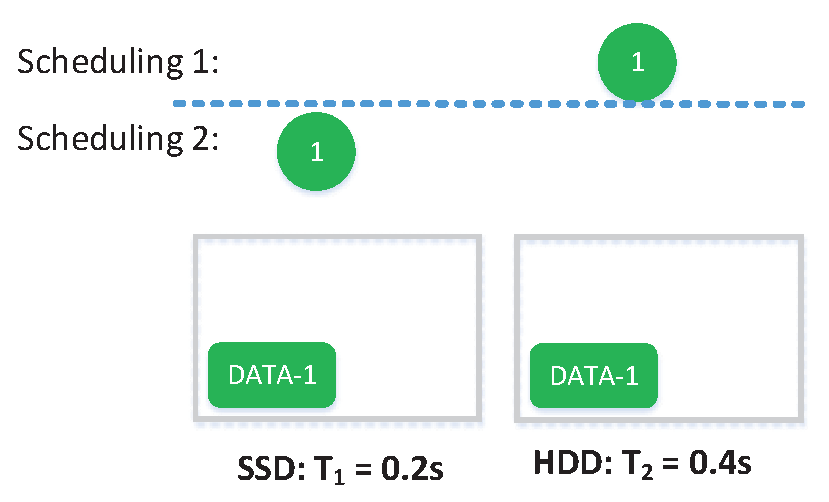
\includegraphics[height=1.1in]{fig_example1_3.eps}}	
%	\subfigure[Load of storage.  Scheduling 1 = $0.2s*3$, Scheduling 2 = $max\{0.2s*2, 0.4s*1\}$]{\label{Fig:example2}
%	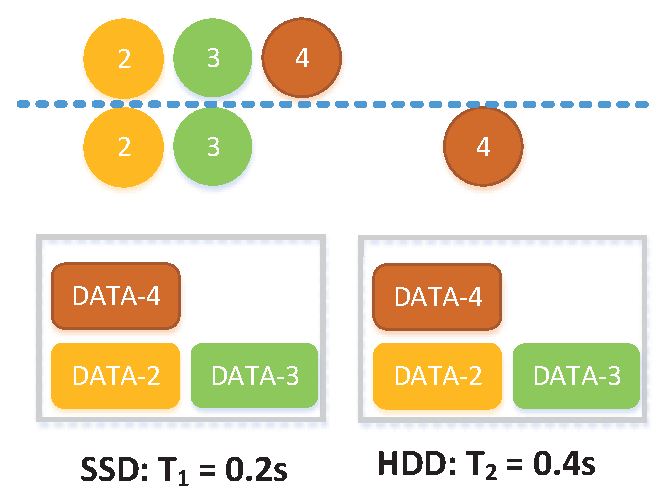
\includegraphics[height=1.1in]{fig_example2_2.eps}}
%	\caption{Two aspects that affect the task completion time: (1) type of storage, \protect\\(2) Load of storage. Delicate method, i.e., Scheduling 2, improves 50\%, 33\% over scheduling 1, respectively.}
%	\label{Fig:example}
%\end{minipage}
%\end{figure}

\begin{figure}[!t]
\centering
    \begin{minipage}{4.78cm}
        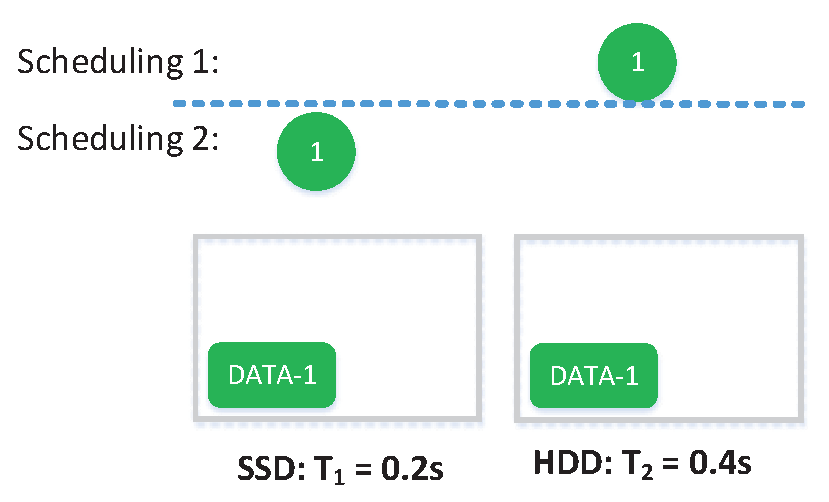
\includegraphics[width=4.78cm]{fig_example1_3.eps}
        \centerline{(a) Type of storage.}\\
        \centerline{Scheduling 1 = $0.4s$,}\\
        \centerline{Scheduling 2 = $0.2s$.}\\
         \centerline{}\\
    \end{minipage}
    \begin{minipage}{3.95cm}
        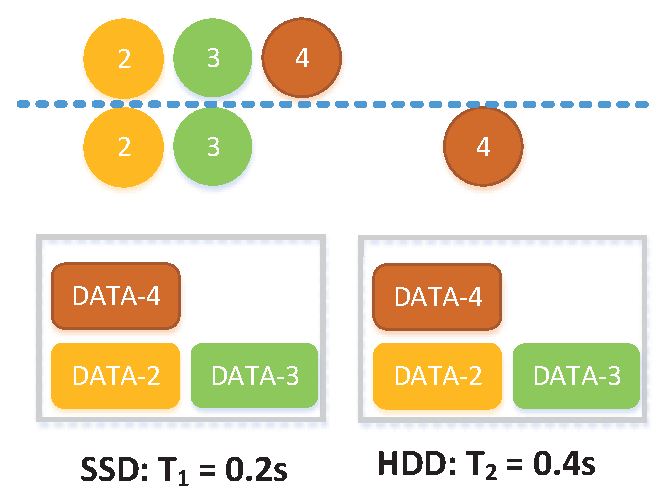
\includegraphics[width=3.95cm]{fig_example2_2.eps}
        \centerline{(b) Load of storage.}\\
        \centerline{Scheduling 1 = $0.2s*3$,}\\
        \centerline{Scheduling 2 = \;\;\;\;\;\;\;\;\;\;\;\;\;}\\
        \centerline{$max$\{$0.2s*2$, 0.4s\}.}\\
    \end{minipage}
    \vspace{-0.4cm}
    \caption{Two aspects that affect the task completion time: (a) type of storage, (b) Load of storage. Delicate method, i.e., Scheduling 2, improves 50\%, 33\% over scheduling 1, respectively.}
    \label{Fig:example}
    \vspace{-0.2cm}
\end{figure}


\subsection{System Model}

The major notations we need are shown in table \ref{table-notations}. The data center is equipped with heterogeneous disks, and we denote by $\mathbb{D}$ the heterogeneous disks set, $\mathbb{D}$ = \{$d_{1}$, $d_{2}$, ...,$d_{|\mathbb{D}|}$\}. $\mathbb{M}$ is defined as the data set in data center, $\mathbb{M}$ = \{$m_{1}$, $m_{2}$, ..., $m_{|\mathbb{M}|}$\}. Each data $m_{l}$ has $C$ replicas whose size $\tau$, e.g., 64MB or 128MB, denoted by \{$r_l^1$, $r_l^2$,... $r_l^{C}$\} stored on $C$ different disks. $\pi_l^{i}$ is a binary variable indicating whether data $m_l$ is stored in disk $d_i$ or not.
If the disk $d_{i}$ stores a replica of the data $m_l$, then $\pi_l^{i}$ = 1. Otherwise, $\pi_l^{i}$ = 0. In data center with heterogeneous disks, each disk $t_i$ has a different time to read a replica, denoted by $T_i$.

When the job arrives, the job will be divided into parallel tasks, denoted by $\mathbb{T}$ = \{$t_1$, $t_2$, ..., $t_{\mathbb{T|}}$ \}. Each task $t_j$ corresponds to one data $\phi(t_j)$, where $\phi(t_j)$ represents data that $t_j$ need. Since there are $C$ replicas for each data deployed in $C$ disks, $t_j$ can read $\phi(t_j)$ from one of the $C$ disks, denoted by \{$d_{j1}$, $d_{j2}$,... $d_{j|C|}$\}.


$I_i^j$ is a decision variable indicating whether task $t_j$ choose to read the replica stored in disk $d_i$ or not. If the task $t_j$ chooses the replica stored in disk $d_i$, then $I_i^j$ = 1. Otherwise, $I_i^j$ = 0. The time of reading a replica for task $t_j$ from disk $d_i$ is $T_i$. Then, we denote by $load_i$ the completion time of all read tasks for the disk $d_i$, $load_{i}$ = $\sum_{j}I_i^j*T_i$. In order to balance the usage of heterogeneous and speed up the completion time of data  analytics, our objective is to minimize the maximum disk load.

\begin{table}[!t]
	\Large
	\centering
	\footnotesize
	\renewcommand\arraystretch{1.2}
	\caption{THE MAJOR NOTATIONS USED IN THIS PAPER.}
	\label{table-notations}
	\begin{tabular}{c|l}
		\hline\hline
		Variable & Notes\\
		\hline
		$d_{i}$ & \tabincell{l}{The disk $i$ and $d_i \in \mathbb{D}$ } \\
		\hline
		$t_{j}$ & \tabincell{l}{The task $j$ and $t_j \in \mathbb{T}$ } \\
		\hline
		$m_{l}$ & \tabincell{l}{The data $l$ and $m_l \in \mathbb{M}$ } \\
		\hline
		$r_{l}^{k}$ & \tabincell{l}{The data replica $k$ of data  $m_l $ } \\
		\hline
		$T_{i}$ & \tabincell{l}{The time required to read \\a replica from disk $d_i$} \\
		\hline
		$\phi(t_j)$ & The data that task $t_j$ needs, and $\phi(t_j)$ $\in$  $\mathcal{M}$ \\
		\hline
		$\pi_{l}^{i}$ & \tabincell{l}{A binary variable indicating if data $m_l$ are \\stored at disk $d_i$ or not} \\
		\hline
		$\phi(t_j)$ & The data that task $t_j$ needs \\
		\hline
		$N_(i)$ & Number of tasks which select data from disk i\\ as input \\
		\hline
		$\tau$ & Size of each data replica in datacenter \\
		\hline
		$C$ & The number of replicas of each data. \\
		\hline\hline
		Decision variable & Notes\\
		\hline
		${I}_i^j$ & \tabincell{l}{A binary variable indicating if task $t_{i}$ choose \\ the replica  that stored in $d_{i}$ as input  or not}\\
		\hline	
	\end{tabular}
\end{table}

\subsection{Heterogeneous Storage-aware Task Scheduling Problem Formulation ($\rm{HTS}$)} \label{HTS}
%$\mathcal{AP} \mathbb{AP}$ (~/~)
A large number of tasks are running in the cluster of data centers. If the scheduler are unaware of the heterogeneity of disks, it is likely that there are a large number of tasks that read data from the same low-speed disk, resulting in bottlenecks. To avoid such situation, we propose heterogeneous storage-aware task scheduling(HTS), as shown below. The optimization goal is to minimize the maximum disk load. Finally, by determining the value of the decision variable $I_i^j$, the appropriate disk is selected for each task to read the corresponding data. Detailed description is as follows:
\begin{align}
Min:&\;\;\;\;\;\max\limits_{i}\{\sum_{j}I_i^j*T_i\}\;\;\;\;\;\;[\rm{HTS}]\nonumber\\
s.t. 
&\;\;\;\;\;\sum_{i}I_i^j = 1,\;\;\forall j,\label{task-cons}\\
&\;\;\;\;\;I_i^j \leq \pi_{\phi(t_j)}^{d_i},\;\;\forall i,j\label{data-cons},\\
&\;\;\;\;\;I_i^j\in\{0,1\},\;\;\forall i,j.\label{def-cons}
\end{align}

Constraint (\ref{task-cons}) guarantees that task $t_j$ can only fetch data $\phi(t_j)$ from one source. Constraint (\ref{data-cons}) guarantees that task $t_j$ can only select from those disks containing its input data. If one replica of data $\phi(t_j)$ is stored in disk $d_i$, then $\pi_{\phi(t_j)}^{d_i}$ = 1, otherwise $\pi_{\phi(t_j)}^{d_i}$ = 0. Constraint 3 denotes the domain of decision variables, which can only be 0 or 1. $I_i^j$ = 1 indicates that task $t_j$ selects the replica stored on disk $d_i$ as input, while task $t_j$ = 0 is on the contrary.

The key to solve HTS problem is to determine the value of decision variables {$I_i^j$}. Next, we show the NP-hardness of this problem. HTS problem can be reduced from the integer linear programming (ILP) problem. The ILP problem is NP-hard, and it follows that HTS problem is NP-hard. The specific proof process is as follows.

\emph{\textbf{Theorem 1:}} The HTS problem is NP-hard.

\emph{Proof:}
The canonical form \cite{b11} of ILP is described below.

For $m\times n$ matrix \textbf{A}
\begin{align}
Min:&\;\;\;\;\;\textbf{c}^T\textbf{x}\;\;\;\;\;\;[\rm{ILP}]\label{ILP}\\
s.t. 
&\;\;\;\;\;\textbf{A}\textbf{x}\geq \textbf{b},\nonumber\\
&\;\;\;\;\;\textbf{x} \geq0\;and\;\textbf{x} \in \mathbb{Z}^n.\nonumber
\end{align}

Taking the special case of HTS problem, the parameters are set as follows:
\begin{itemize}
	\item $\mathbb{D}$ = \{$d_0$, $d_1$, $d_2$\};$T_0$ = 1, $T_1$ = 1, $T_2$=1; $\mathbb{M}$ = \{$m_0$, $m_1$, ..., $m_{n-1}$\}; $C$ = 3
	\item $T$ = \{$t_0$, $t_1$, ..., $t_{n-1}$\}
\end{itemize}

It means that there are 3 disks, $d_0$, $d_1$, $d_2$, in the data center, each disk with a $T_i$ of 1. A total of n data, and each data has three replicas which deployed in the three disks, respectively. When the query job arrives, the job is divided into n tasks, $t_0$, $t_1$, ..., $t_n$ to read n data,$m_0$, $m_1$, ..., $m_n$, respectively.

For this particular case, the problem description can be modified to:

\begin{align}
Min:&\;\;\;\;\;\max\{\sum_{j}I_0^j, \sum_{j}I_1^j, \sum_{j}I_2^j\}\;\;\;\;\;[\rm{HTS-sp}]\\
s.t. 
&\;\;\;\;\;I_0^j + I_1^j +I_2^j= 1,\;\;\forall j,\nonumber\\
&\;\;\;\;\;I_0^j, I_1^j, I_2^j\in\{0,1\},\;\;\forall j \in[0,n).\nonumber
\end{align}

Let  $x$ = $\sum_{j}I_0^j$, $y$ = $\sum_{j}I_1^j$, $z$ = $\sum_{j}I_2^j$, and the problem description can be modified to:
\begin{align}
Min:&\;\;\;\;\;\max\{x,y,z\}\;\;\;\;\;\;[\rm{HTS-sp}]\\
s.t. 
&\;\;\;\;\;x + y + z = n,\;\label{enlarge-cons}\\
&\;\;\;\;\;0 \leq x, y, z \leq n  \;\;x, y, z\in\mathbb{Z}.\nonumber
%&\;\;\;\;\;0 \leq y \leq n, y\in\mathbb{Z}\nonumber\\
%&\;\;\;\;\;0 \leq z \leq n, z\in\mathbb{Z}\nonumber
\end{align}
In the minimization problem, x + y + z = n can be modified to x + y + z = n and let $R$ denotes $\max\{x,y,z\}$. 

Finally, HTS-sp problem is converted to:
\begin{align}
Min:&\;\;\;\;\;0*x+0*y+0*z+R\;\;\;\;\;\;\;[\rm{HTS-ILP}]\label{HTS-ILP}\\
s.t. 
&\;\;\;\;\;x + y + z \geq n,\;\nonumber\\
&\;\;\;\;\;-x + R \geq 0, \nonumber\\
&\;\;\;\;\;-y + R \geq 0, \nonumber\\
&\;\;\;\;\;-z + R \geq 0, \nonumber\\
&\;\;\;\;\;0 \leq x, y, z \leq n  \;\;x, y, z\in\mathbb{Z},\nonumber\\
%&\;\;\;\;\;0 \leq x \leq n, x\in\mathbb{Z}\nonumber\\
%&\;\;\;\;\;0 \leq y \leq n, y\in\mathbb{Z}\nonumber\\
%&\;\;\;\;\;0 \leq z \leq n, z\in\mathbb{Z}\nonumber\\
&\;\;\;\;\;R \geq 0, R\in\mathbb{Z}.\nonumber
\end{align}

Obviously, HTS-ILP in (\ref{HTS-ILP}) is an instance of ILP in (\ref{ILP}). The decision version of 0-1 ILP (A variation in which only the restrictions must be satisfied, without optimization) is one of Karp's 21 NP-complete problems  \cite{b9}, so ILP is NP-hard. Further, the HTS-ILP problem is NP-hard.

On the one hand, when the optimal solution of HTS-ILP problem is obtained, the corresponding {x, y, z} can be converted into variable {$I_i^j$} in polynomial time by setting the value in \{$I_0^0$, $I_0^1$, ...,$I_0^{x-1}$, $I_1^{x}$, $I_1^{x+1}$, ..., $I_1^{x+y-1}$, $I_2^{x+y}$, $I_1^{x+y+1}$, ..., $I_2^{x+y+z-1}$\} to be 1, which will make the corresponding HTS-sp problem obtain the optimal solution. On the other hand, when the variable \{$I_i^j$\} make the HTS-sp problem obtain the optimal solution, the HTS-ILP also obtains the optimal solution by setting $x$ = $\sum_{j}I_0^j$, $y$ = $\sum_{j}I_1^j$, $z$ = $\sum_{j}I_2^j$. It can be seen from the above that any solution can be polynomially transformed between the HTS-sp and HTS-ILP. Therefore, HTS-sp is NP-hard. 

As a result of that HTS-sp is a special case in HTS, HTS problem is NP-hard.\hfill $\qedsymbol$

\section{DESIGN of ALGORITHMS FOR HTS PROBLEM}\label{DESIGN_ALGORITHM}

Due to the hardness of HTS problem, the optimal solution can not be obtained in polynomial time. In order to solve NP-hard problem, we propose a heuristic algorithm based on greedy idea, named HTS-greedy. However, this kind of algorithm usually has no guarantee of quality, although in some cases the solution is not bad, in some cases it is opposite. Furthermore, we design a quality assurance algorithm HTS-rdm, which makes the feasible solution approach to the optimal solution with probability 1- O($e^{-t^2}$) where t is the difference between the solution found by HTS-rdm and optimal solution.


\subsection{Heuristic Alogrithm}\label{Heuristic}

In this subsection, we will introduce the heuristic algorithm HTS-greedy specificly. Using the greedy idea, the HTS-greedy chooses the disk which stores $\phi(t_j)$ for each task $t_j$ and which has the minimum load, and finally outputs one disk for each task.


%Alogoritm1
\begin{algorithm}

	\textbf{Require:} For each task $t_j$, decide a disk $d_i$ that stores one replica of data $\phi(t_j)$.

	\begin{algorithmic}[1]
		\For{each disk $d_i$} \label{HTS-greedy:init}
			\State $load_{i}$ $\gets$ 0
		\EndFor
		\State $Result$ $\gets$ \{\}
		\For{each task $t_j$} 
			\State $d_{j1}$, $d_{j2}$,... $d_{j|C|}$ = $f(\phi(t_j))$
		
			$//$Function $f$ is a mapping from data to disks that stores each replica of the data.
			\State $load_{j_{min}}$ $\gets$ $\min\limits_{l}$($load_{j_l}$)
			
			$load_{j_{min}}$ $\gets$ $load_{j_{min}}$ + $T_{j_{min}}$
			\State Result $\gets$ $Result$ $\cup$
			\{$\left \langle t_j, d_{j_{min}}\right \rangle$\}
		\EndFor
	
	\State \textbf{Return} $Result$
	\end{algorithmic}
	\caption{HTS-greedy}\label{HTS-greedy}
\end{algorithm}

Algorithm \ref{HTS-greedy:init} shows the detailed of HTS-greedy. Line 1-4 initializes $load_i$ = 0 and Result = \{\}, and $load_i$ denotes the total load of the $disk_i$. Line 5-9 is to select a disk for each task $t_j$. In line 6, function f is used to help task $t_j$ find all disks that store replicas of data $\phi(t_j)$. Let $d_{j1}$, $d_{j2}$,... $d_{j|C|}$ denote the $C$ disks. Next, in line 7, the disk with minimum total load is selected from the $C$ disks, and the read time caused by task $t_j$ is added to the $load_i$. Then put the task $t_j$ and disk $d_{j_l}$ into the set Result. After one iteration, the algorithm completes the decision for a task and it needs $\mathbb{T}$ iteration in total.

%Next, an example is given to illustrate the algorithm. In datacenter, there exits a set of heterogeneous disks $\mathbb{D}$= \{$d_1$, $d_2$, $d_3$, $d_4$\} with $T_i$ $T_1$ = 0.3,  $T_2$ = 0.1,  $T_3$ =0.2 and $T_4$ =0.2, respectively. Data set $\mathbb{M}$ = \{$m_1$, $m_2$, $m_3$, $m_4$\} are stored as Fig.\ref{fig1}. Obviously, each data has two replicas. When query tasks $\mathbb{T}$= \{$t_1$, $t_2$, $t_3$, $t_4$\} ($\phi(t_j)$ = j, 1$\leq$j$ \leq$4) comes, the algorithm HTS-greedy runs as follows: %($\phi(t_j)$ = j (1 $\leq$j$ \leq$ 4, task $t_j$'s input is $m_j$ which equals the DATA-j in Fig.\ref{fig1}))

Next, an example is given to illustrate the algorithm. In datacenter, there exits a set of heterogeneous disks $\mathbb{D}$= \{$d_1$, $d_2$, $d_3$, $d_4$\} with $T_1$ = 0.2,  $T_2$ = 0.25,  $T_3$ =0.4 and $T_4$ =0.6, respectively. Data set $\mathbb{M}$ = \{$m_1$, $m_2$, $m_3$, $m_4$\} are stored as Fig.\ref{fig1}. Obviously, each data has two replicas. When query tasks $\mathbb{T}$= \{$t_1$, $t_2$, $t_3$, $t_4$\} ($\phi(t_j)$ = j, 1$\leq$j$ \leq$4) comes, the algorithm HTS-greedy runs as follows: %($\phi(t_j)$ = j (1 $\leq$j$ \leq$ 4, task $t_j$'s input is $m_j$ which equals the DATA-j in Fig.\ref{fig1}))
Initial: Reslut = \{\}, $load_1$=0, $load_2$=0, $load_3$=0, $load_4$=0
\begin{itemize}
	\item \textbf{Round 1}:for task  $t_1$:
	 f($\phi(t_1)$) = \{3, 4\} = \{DISK3, DISK4\}\\
	 $load_3$ = $\min$\{$load_3$ = 0, $load_4$ = 0\}\\
	 $load_3$ = $load_3$ + $T_3$ = 0.4\\
	Result = Result $\cup$ $\left \langle t_1, d_{3}\right \rangle$ = \{$\left \langle t_1, d_{3}\right \rangle$\}
	\item \textbf{Round 2}:for task  $t_2$:
	f($\phi(t_2)$) = \{1, 2\}\\
	$load_1$ = $\min$\{$load_1$ = 0, $load_2$ = 0\}\\
	$load_1$ = $load_1$ + $T_1$ = 0.2\\
	Result = Result $\cup$ $\left \langle t_2, d_{1}\right \rangle$ = \{$\left \langle t_1, d_{3}\right \rangle$, $\left \langle t_2, d_{1}\right \rangle$\}
	\item \textbf{Round 3}:for task  $t_3$:
	f($\phi(t_3)$) = \{1, 3\}\\
	$load_2$ = $\min$\{$load_1$ = 0.2, $load_2$ = 0\}\\
	$load_2$ = $load_2$ + $T_2$ = 0.25\\
	Result = Result $\cup$ $\left \langle t_3, d_{2}\right \rangle$ = \{$\left \langle t_1, d_{1}\right \rangle$, $\left \langle t_2, d_{2}\right \rangle$,  $\left \langle t_3, d_{2}\right \rangle$\}
	\item \textbf{Round 4}:for task  $t_4$:
	f($\phi(t_4)$) = \{1, 2\}\\
	$load_1$ = $\min$\{$load_1$ = 0.2, $load_2$ = 0.25\}\\
	$load_1$ = $load_1$ + $T_1$ = 0.4\\
	Result = Result $\cup$ $\left \langle t_4, d_{2}\right \rangle$ = \{$\left \langle t_1, d_{3}\right \rangle$, $\left \langle t_2, d_{1}\right \rangle$,  $\left \langle t_3, d_{2}\right \rangle$, $\left \langle t_4, d_{1}\right \rangle$\}
	
	\item \textbf{Round 5}:for task  $t_5$:
	f($\phi(t_5)$) = \{1, 2\}\\
	$load_2$ = $\min$\{$load_1$ = 0.4, $load_2$ = 0.25\}\\
	$load_2$ = $load_2$ + $T_2$ = 0.5\\
	Result = Result $\cup$ $\left \langle t_5, d_{2}\right \rangle$ = \{$\left \langle t_1, d_{3}\right \rangle$, $\left \langle t_2, d_{1}\right \rangle$,  $\left \langle t_3, d_{2}\right \rangle$, $\left \langle t_4, d_{1}\right \rangle$, $\left \langle t_5, d_{2}\right \rangle$\}
	\item \textbf{Round 6}:for task  $t_6$:
	f($\phi(t_6)$) = \{1, 2\}\\
	$load_1$ = $\min$\{$load_1$ = 0.4, $load_2$ = 0.5\}\\
	$load_1$ = $load_1$ + $T_1$ = 0.6\\
	Result = Result $\cup$ $\left \langle t_6, d_{1}\right \rangle$ = \{$\left \langle t_1, d_{3}\right \rangle$, $\left \langle t_2, d_{1}\right \rangle$,  $\left \langle t_3, d_{2}\right \rangle$, $\left \langle t_4, d_{1}\right \rangle$, $\left \langle t_5, d_{2}\right \rangle$, $\left \langle t_6, d_{1}\right \rangle$\}
	
	
	
\end{itemize}
\begin{figure}[!t]
	\centering
	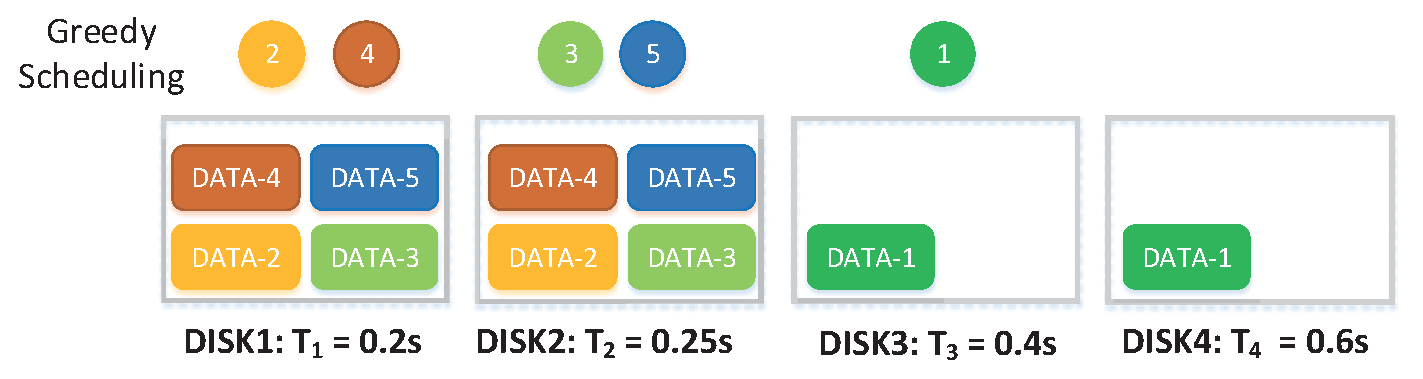
\includegraphics[height=0.8in]{fig1_8.eps}
	\caption{An execution example of greedy algorithm  }
	\label{fig1}
\end{figure}
\begin{figure}[!t]
	\centering
	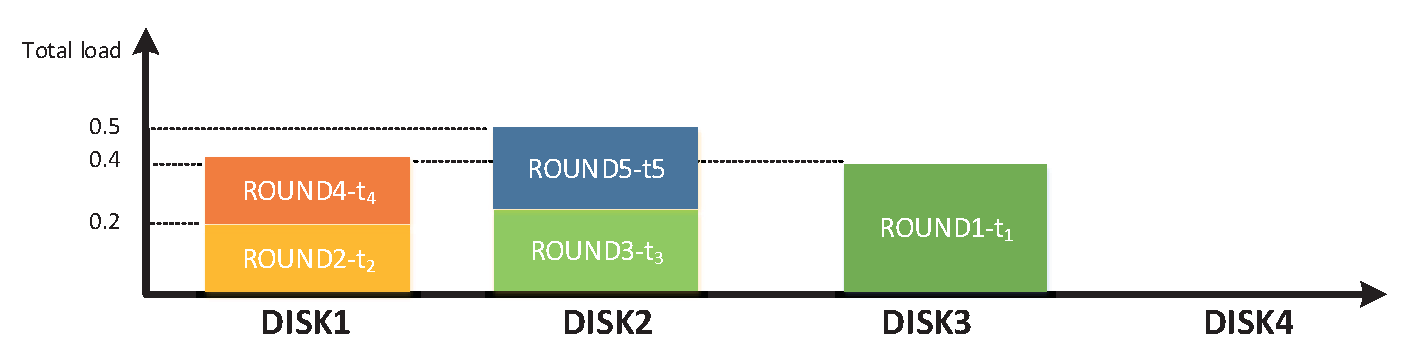
\includegraphics[height=0.8in]{fig2_1.eps}
	\caption{The process of HTS-greedy algorithm execution for the data stored as Fig.\ref{fig1}. }
	\label{fig2}
\end{figure}

The final result is in Result and  Tasks will follow \{$\left \langle t_1, d_{3}\right \rangle$, $\left \langle t_2, d_{1}\right \rangle$,  $\left \langle t_3, d_{2}\right \rangle$, $\left \langle t_4, d_{1}\right \rangle$, $\left \langle t_5, d_{2}\right \rangle$, $\left \langle t_6, d_{1}\right \rangle$\} to read data.The specific process of HTS-greedy algorithm is shown in Fig.\ref{fig2}.

\subsection{Randomized Alogrithm}\label{Randomized}

In the previous section \ref{Heuristic}, we designed a greedy heuristic algorithm HTS-greedy to solve HTS problems. However, this algorithm does not have performance guarantee. Therefore, in this subsection, we propose a performance-guaranteed random algorithm HTS-rdm. By relaxing the HTS problem to HTS-relaxation problem, HTS-rdm uses linear programming to solve HTS-relaxation. The decomposition obtained by linear programming is a fraction rather than an integer, which represents the preference when selecting disks. Subsequently, we prove that the solution found by the HTS-rdm algorithm can approach the optimal solution with probability 1- O($e^{-t^2}$) where t is the difference between the solution found by HTS-rdm and optimal solution..

\paragraph{\textbf{Relaxation of HTS Problem}} According to the previous analysis \ref{HTS}, this problem is NP-hard, which cannot be solved in polynomial time. But the linear programming (LP) problem is solvable in polynomial time, a natural point of view is to relax the HTS problem to LP. The method is to change the range of variables from integer domain \{0, 1\} to real domain [0, 1]. As shown below, HTS-relaxtion, this process is named \textbf{relaxation}. The solution of HTS-relaxtion provides a lower bound for the original HTS problem (HTS is a minimization problem. For the maximization problem is on the contrary). Next, based on the solution of linear programming, the fractional solution is mapped back to integer in some way, which is named \textbf{rounding}. Based on relaxation-rounding, we propose HTS-rdm algorithm.

 \begin{align}
 Min:&\;\;\;\;\;\max\limits_{i}\{\sum_{j}p_i^j*T_i\}\;\;\;\;\;\;[\rm{HTS-relaxtion}]\nonumber\\
 s.t. 
 &\;\;\;\;\;\sum_{i}p_i^j = 1,\;\;\forall j,\nonumber\\
 &\;\;\;\;\;p_i^j \leq \pi_{\phi(t_j)}^{d_i},\;\;\forall i,j,\nonumber\\
 &\;\;\;\;\;p_i^j \in[0, 1],\;\;\forall i,j.\nonumber
 \end{align}
 
 The detailed procedure of HTS-rdm algorithm is shown in Algorithm \ref{HTS-rdm}. Line 1 initializes the Result set, which stores the final result. In the second line, the HTS-relaxation problem is solved by linear programming tools. The third line uses rounding strategy to convert fractional solution to integer solution. Line 4-9 organize the results and output them. Then the task will read the disk according to the results. The specific rounding strategies are as follows:
 
 The value of \{$p_i^j$\}  $\in$ [0, 1] which shows the correlation between task $t_j$ and disk $d_i$. Therefore, we can select disk $d_i$ for task $t_j$ with  probability \{$p_i^j$\}. The method is to use the parameter $q_j$, which is randomly selected in (0,1]. If the $q_j$ $\in$ ($\sum p_{r-1}^{j}$, $\sum p_{r}^{j}$], then $I_r^j = 1$, otherwise, $I_i^j$ = 0 ($\forall$ $i$, $i \ne r$). This approach ensures only one disk can be selected for each task.%For each task $t_j$, the corresponding decision variables are \{$p_0^j$,$p_i^j$, ..., $p_i^j$\}. 
 \begin{algorithm}
 	%\renewcommand{\thealgorithm}{}
 	
 	\textbf{Require:} Decide a disk $d_i$ for each task $t_j$. %and $d_i$ stores data $\phi(t_j)$.
 	\begin{algorithmic}[1]
 		
 		\State Result $\gets$ \{\}
 		\State \{$p_i^j$\} = HTS-relaxtion		
 		$//$ is the solution of HTS-relaxtion problem. 
 		
 		\State Based on \{$p_i^j$\}, use rounding strategy and get \{$I_i^j$\}
 		\For{$\forall$ $i$, $j$}  
 			\If{$I_i^j$ == 1}
 			\State Result $\gets$ Result $\cup$ 	
 			\{$\left \langle t_j, d_i\right \rangle$\}
 			\EndIf
 		\EndFor	
 		\State \textbf{Return} Result	
 	\end{algorithmic}
 	\caption{HTS-rdm}\label{HTS-rdm}
 \end{algorithm}

\paragraph{\textbf{Analysis of HTS-rdm Algorithm}}

In this section, we will prove that the HTS-rdm algorithm can approach the optimal solution with a probability 1- O($e^{-t^2}$). Firstly, we prove that the difference between read time contributed by any tasks $t_j$ to $d_i$ and expectation is matingales sequence \cite{b12}. Secondly, Based on the matigales sequence, we use Azuma inequality to illustrate the bound between the feasible solution and the optimal solution.
\begin{figure*}[!t]
	\centering
	\subfigure[Small Workload ]{\label{Fig:instance1}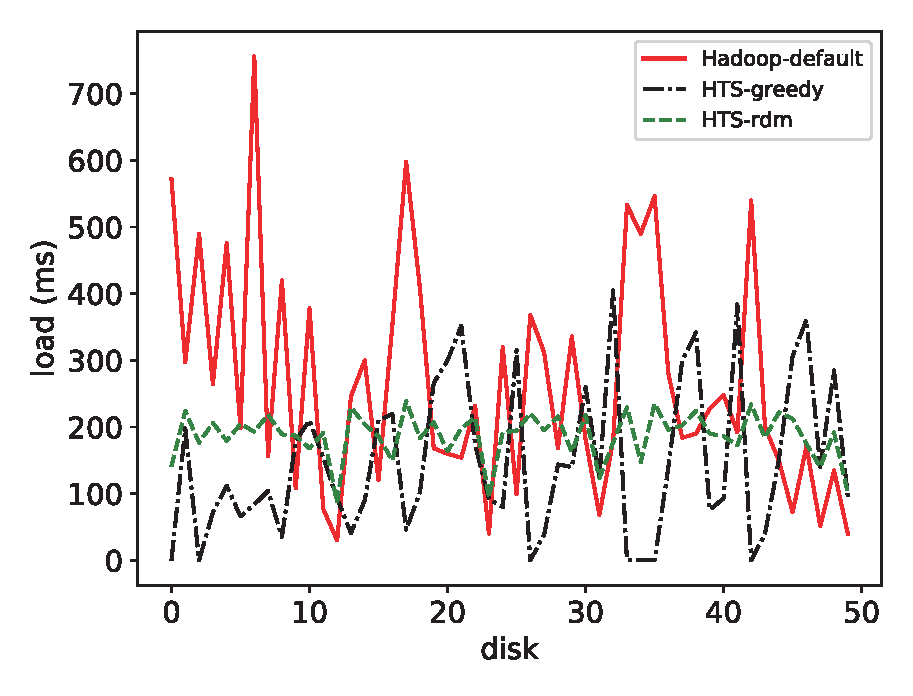
\includegraphics[height=1.6in]{fig_instance1_3.eps}}\quad\quad %quad 表示图像的间距
	\subfigure[Medium Workload ]{\label{Fig:instance2}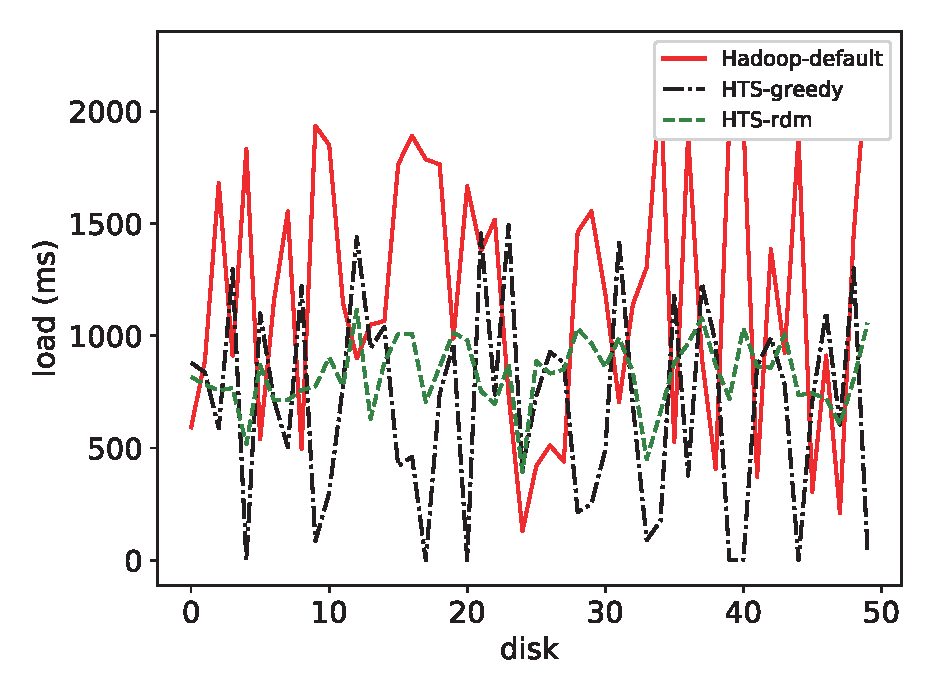
\includegraphics[height=1.6in]{fig_instance2_3.eps}}\quad\quad
	\subfigure[Large Workload
	]{\label{Fig:instance3}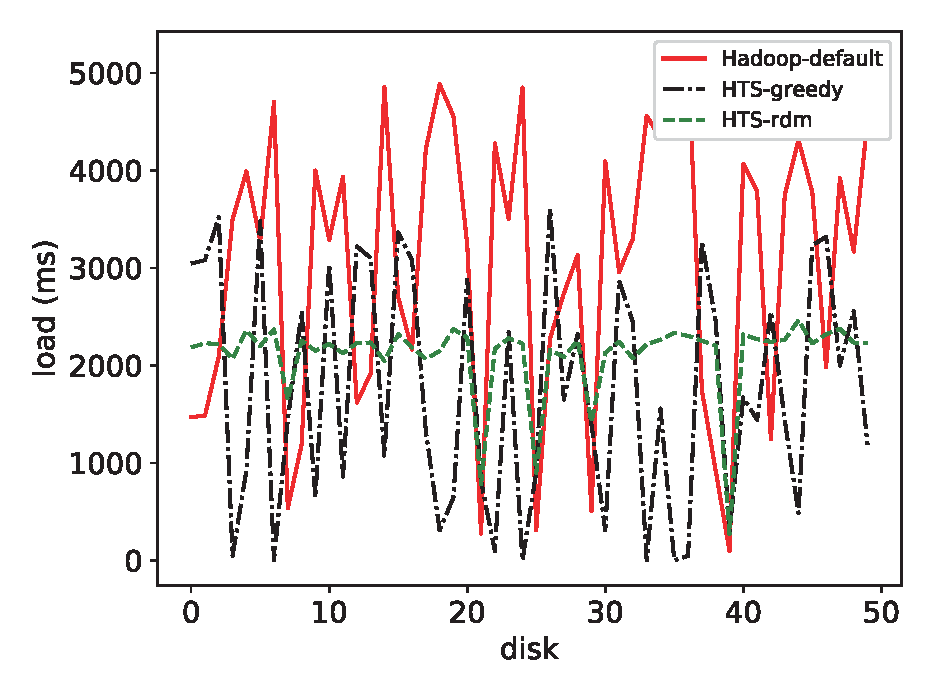
\includegraphics[height=1.6in]{fig_instance3_3.eps}}
	\vspace{-1ex}
	\caption{Comparison of HTS-rdm and other Algorithm on different Workloads. \ref{Fig:instance1} denotes the results on Small Workload which has about 500 tasks. \ref{Fig:instance2} denotes the results on Medium Workload which has about 2000 tasks.
	\ref{Fig:instance3} denotes the results on Large Workload which has 5000 tasks. X-axis denotes the disk. Y-axis denotes the load of each disk after running the three algorithms.}
	\label{Fig:instance}
	\vspace{-1ex}
\end{figure*}


\emph{\textbf{Theorem 2:}} $Pr[SOL(HTS-rdm) - OPT(HTS) \leq t] \geq 1 - O(e^{-t^2})$.

\emph{\textbf{Proof:}}

$SOL(HTS-rdm)$ denotes the feasible solution found by HTS-rdm algorithm and  $OPT(HTS)$ denotes the optimum solution of HTS problem.

Firstly, task $t_j$'s contribution to disk $d_i$'s load is expressed as:
 \begin{align}
&\;\;\;\;\;Z_i^j = I_i^j*T_i
\end{align}

From the rounding strategy in Algorithm \ref{HTS-rdm}, we can get that:
 \begin{align}
&\;\;\;\;\;Pr[I_i^j = 1] = p_i^j,\;\;for\forall i,j \nonumber
\end{align}
%Therefore

The expectation of $Z_i^j$ is
\begin{align}
E[Z_i^j] &\;\;\;= E[I_i^j]*T_i \nonumber\\
&\;\;\;= (Pr[I_i^j = 1] * 1 + Pr[I_i^j = 0] * 0)*T_i \nonumber\\
&\;\;\;= p_i^j*T_i\label{prove:expect}
\end{align}

The difference between $Z_i^j$ and $E[Z_i^j]$ defines as
\begin{align}
Q_i^j = Z_i^j - E[Z_i^j]\label{prove:diff}
\end{align}

For the all $\mathbb{|T|}$ tasks, $L_i^{\mathbb{|T|}}$ denotes the sum of $Q_i^j$ in disk $d_i$:
\begin{align}
L_i^{\mathbb{|T|}} = \sum_{j = 1}^{\mathbb{|T|}} Q_i^j
= \sum_{j = 1}^{\mathbb{|T|} - 1} L_i^j + Q_i^{\mathbb{|T|}} \label{prove:L_margin}
\end{align}
Then, on the condition $L_i^{1}$, $L_i^{2}$, ..., $L_i^{r-1}$, the expectation of $L_i^{r}$ is:
\begin{align}
&E[L_i^{r}|L_i^{1}, L_i^{2}, ..., L_i^{r-1}] \nonumber\\
&\overset{\text{(\ref{prove:L_margin})}}{=}E[L_i^{r-1} + Q_i^{r} |L_i^{1}, L_i^{2}, ..., L_i^{r-1}] \nonumber\\
&\overset{\text{}}{=}E[L_i^{r-1} |L_i^{1}, L_i^{2}, ..., L_i^{r-1}]
+ E[Q_i^{r} |L_i^{1}, L_i^{2}, ..., L_i^{r-1}] \nonumber\\
&\overset{\text{(\ref{prove:diff})}}{=}L_i^{r-1} + E[Z_i^r - E[Z_i^r] |L_i^{1}, L_i^{2}, ..., L_i^{r-1}]\nonumber\\
&=L_i^{r-1} + E[Z_i^r|L_i^{1}, L_i^{2}, ..., L_i^{r-1}]
-E[E[Z_i^r] |L_i^{1}, L_i^{2}, ..., L_i^{r-1}]\nonumber\\
&=L_i^{r-1} + E[Z_i^r] - E[Z_i^r]\nonumber\\
&=L_i^{r-1}\label{prove:marginsq}
\end{align}
Therefore, $L_i^{1}$, $L_i^{2}$, ..., $L_i^{|\mathbb{T}|}$ are matigales sequence \cite{b13}. For completeness, we let $L_i^{0}$ = 0. And for $\forall r \geq 1$, we have:
\begin{align}
  |L_i^r - L_i^{r-1}|\overset{\text{(\ref{prove:L_margin})}}{=} |Q_i^{r}| \overset{\text{(\ref{prove:diff})}}{=} |Z_i^j - E[Z_i^j]|\leq g_i^r\\
  g_i^r = \max\{T_i -  E[Z_i^j], E[Z_i^j]\}\label{prove:bound}
\end{align}

From above (\ref{prove:bound}), any two adjacent values $L_i^r$, $L_i^{r-1}$ in the margingales sequence have constant bounds $g_i^r$. Based on (\ref{prove:marginsq}) and (\ref{prove:bound}), we can use Azuma's inequality. Then, 

\begin{align}
Pr\{L_i^{|\mathbb{T}|} - L_i^{0} \geq t\} \leq exp\{-\frac{t^2}{2\sum_{ i = 1 }^{|\mathbb{T}|}(g_i^k)^2}\} \label{prove:azuma}
\end{align}

Substitute equations (\ref{prove:diff}) and (\ref{prove:L_margin}) into the upper equation (\ref{prove:azuma}). Then, 

\begin{align}
Pr\{\sum_{j = 1}^{|\mathbb{T}|} Z_i^j - 
	\sum_{j = 1}^{|\mathbb{T}|} E[Z_i^j]\geq t\} \leq exp\{-\frac{t^2}{2\sum_{ i = 1 }^{|\mathbb{T}|}(g_i^k)^2}\} \label{prove:azuma1}
\end{align}
 The (\ref{prove:azuma1}) is equal to:
\begin{align}
Pr\{\sum_{j = 1}^{|\mathbb{T}|} Z_i^j \leq \sum_{j = 1}^{|\mathbb{T}|} E[Z_i^j] + t\} \geq 1 - exp\{-\frac{t^2}{2\sum_{ i = 1 }^{|\mathbb{T}|}(g_i^k)^2}\}\nonumber\\
= 1 - O(e^{-t^2})\label{prove:azuma3}
\end{align}

Let $S_i$  = $\sum_{j = 1}^{|\mathbb{T}|} Z_i^j$,
$E_i$ = $\sum_{j = 1}^{|\mathbb{T}|} E[Z_i^j]$
$\overset{\text{(\ref{prove:expect})}}{=}$
$\sum_{j = 1}^{|\mathbb{T}|} p_i^j*T_i$. Then,
\begin{align}
Pr\{S_i \leq U_i + t\} \geq 1- O(e^{-t^2}) \label{prove:SU}
\end{align}

$S_i$ denotes the load of disk $d_i$ which is the result of ILP. And $E_i$ denotes the expectation which is the result of LP. Because LP provides a lower bound for the optimal solution of ILP problem (HTS is a minimization problem. For the maximization problem is on the contrary), we have:



\begin{align}
E_i \leq OPT(HTS)\label{prove:OPT}
\end{align}

Take $S_u$, $E_v$ as
\begin{align}
	S_u = S_{max} = \max_i S_i\\
	E_v = E_{max} = \max_i E_i\label{prove:Emax}
\end{align}

Then, we have the following inequalities,
\begin{align}
SOL(HTS-rdm) = S_u  
\overset{\text{(\ref{prove:azuma3})}}{\leq}  E_u+t
\overset{\text{(\ref{prove:Emax})}}{\leq} E_v+t\nonumber\\
\overset{\text{(\ref{prove:OPT})}}{\leq} OPT(HTS)+t\label{prove:SOL-OPT}
\end{align}

From (\ref{prove:SU}) and (\ref{prove:SOL-OPT}), we can conclude that,
\begin{align}
Pr\{SOL(HTS-rdm)<OPT (HTS)+t\} \geq 1 - O(e^{-t^2})\label{prove:result}
\end{align}

Observed from the (\ref{prove:result}), the feasible solution $SOL(HTS-rdm)$ found by the algorithm and the optimal solution OPT (HTS) are approximated by probability $1 - O(e^{-t^2})$. When hundreds of tasks are deployed with $1 - O(e^{-t^2})$ = 0.85, the value of $t$ is acceptable, only a few millisecond.\hfill $\qedsymbol$


\section{PERFORMANCE EVALUATION}\label{PERFORMANCE_EVALUATION}

In this section, we implement our algorithms HTS-greedy and HTS-rdm, and compare our algorithms with storage-unaware scheduling algorithm. The results show that performance can be improved by 40\%.
\subsection{Simulation Settings}\label{SCM}
Usually, the general scheduling mechanism are not aware of the heterogeneity of the disk. For example, in Hadoop the scheduler cannot know the load of the disk when deploying the task. When selecting data replica for tasks, it is usually a random selection strategy, which we call Hadoop-default. We compare our proposed algorithms with it.

\textbf{Workload:} Referring to the characteristics of Google traces \cite{b20}, we classify workload into three categories: Small Workload, Medium Workload and Large Workload, as shown in TABLE \ref{tab:workload}. In Small Workload, most of the jobs have 1-150 tasks. In has Large Workload, there are 50\% of the jobs that has over 50 tasks. The Medium Workload is in the middle of them.

\begin{table}[htbp]
	\caption{THE DIFFERENT TRACES USED FOR EXPERIMENT}
	\begin{center}
		\begin{tabular}{|c|c|c|c|}
			\hline
			 \diagbox{Traces}{Number of tasks} & 1-150 & 150-500 & $\ge$ 500\\
			\hline
			Small Workload & 96\% & 2\% & 2\%\\
			\hline
			Medium Workload & 50\% & 40\% & 10\%\\
			\hline
			Large Workload & 40\% & 10\% & 50\%\\
			\hline
		\end{tabular}
		\label{tab:workload}
	\end{center}
\end{table}

\textbf{Setting:}
In distributed file systems \cite{b19}, data is distributed uniformly on disk. Therefore, in this experimental environment, we uniformly deploy 200000 data with three data replicas by default, each data block size $\tau$ = 128MB. 500 disks are set up by default. The $T_i$ of the disk in the cluster is between 10 and 500 in ms. 


\begin{figure*}[!t]
	\centering
	\subfigure[Results under varilous setting on Workloads ]{\label{Fig:completeWorkload}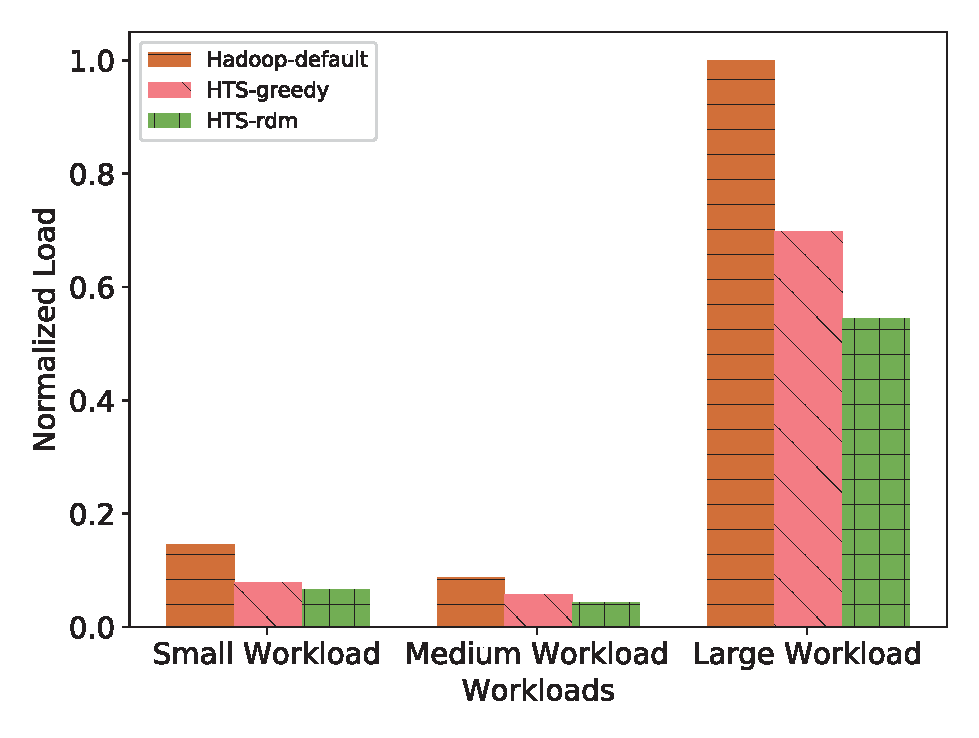
\includegraphics[height=1.6in]{figcomplete1_4.eps}}\quad\quad %quad 表示图像的间距
	\subfigure[Results under different Heterogeneity cluter. ]{\label{Fig:completeHeter}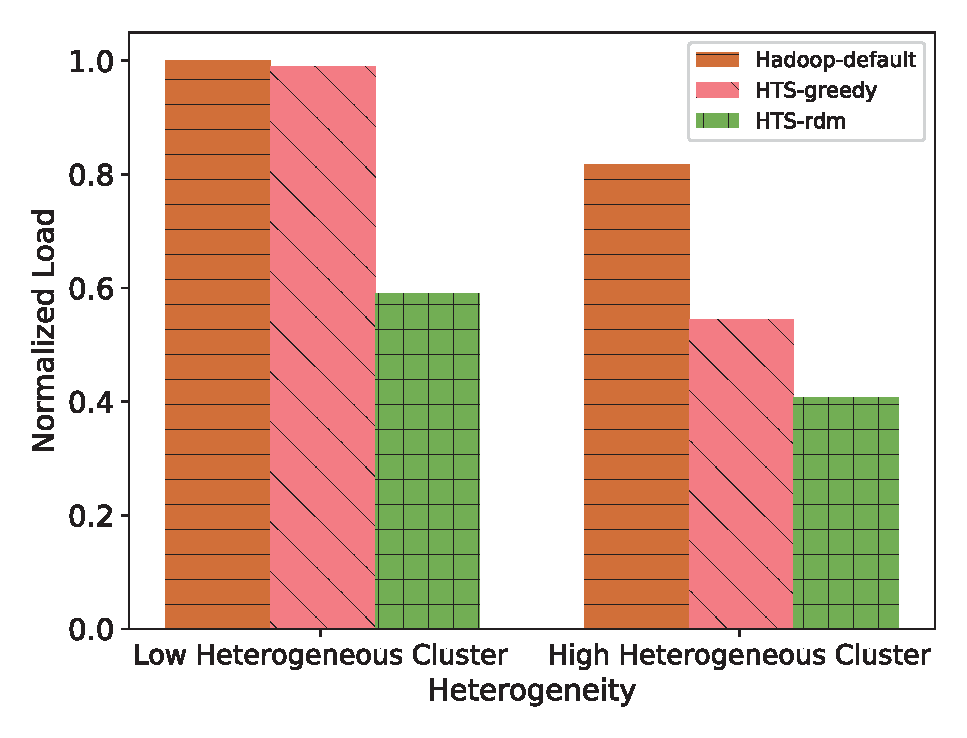
\includegraphics[height=1.6in]{figcomplete2_4.eps}}\quad\quad
	\subfigure[Results under varilous setting on reolicas number
	]{\label{Fig:completeRep}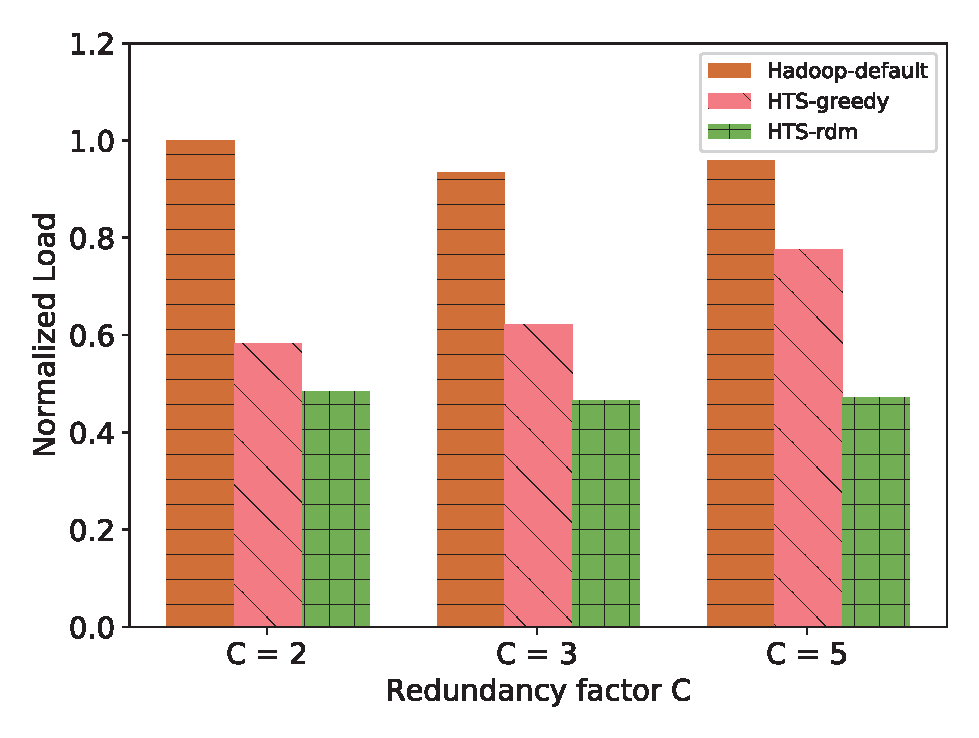
\includegraphics[height=1.6in]{figcomplete3_4.eps}}
	\vspace{-1ex}
	\caption{Comparison of HTS-rdm and other Algorithm on different workloads, different heterogenelity cluter and different replica number $C$. \ref{Fig:completeWorkload} denotes effect of different workloads on completion time. \ref{Fig:completeHeter} denotes the completion time of the three algorithm on different Heterogeneity cluter. \ref{Fig:completeRep} denotes the completion time of the three algorithm when $C$ is different. Y-axis denotes the completion time of all tasks which has been normalized.}
	\label{Fig:complete}
	\vspace{-3ex}
\end{figure*}

\subsection{Simulation Results}

For convenience of display, Fig.\ref{Fig:instance}. shows the results under different workloads upon 50 disks. X-axis denotes the disks. Y-axis denotes the load of each disk after running the three algorithms. The lower the peak of the curve, the better the result. The black dotted line represents the execution result of Algorithm HTS-greedy, and the green line represents the execution result of Algorithm HTS-rdm. Overall, we can see that our algorithm performs better than Hadoop-default. As shown in Fig.\ref{Fig:instance1}, in the small workload, the result of Hadoop-default has large fluctuations. This is a result of that hadoop-default is not aware of the $T_i$ and load of the disk when selecting a replica for the task. Even if the tasks are deployed uniformly on disks, the disk with low performance may have a relatively large load. In Fig. \ref{Fig:instance1}, low performance disks will have high peaks. Completion of all parallel tasks is the end of the big data processing job. Therefore, the task reading data from the disk with poor performance will be the bottleneck of data processing job. For example, Hadoop-default causes the tasks of reading data from disk-2 to be the bottleneck of big data processing in the Fig.\ref{Fig:instance1} which is 654. Algorithms HTS-greedy and HTS-rdm can maintain roughly all disks at a lower load, less than 300. The reason is that HTS-greedy can select the disk to read for the task according to load of the disks and HTS-rdm can select the disk to read for the task according to load of the disks the performance of the disk. The maximum load of HTS-greedy algorithm is 261 in disk-12. Compared with the Hadoop-default, the performance is improved by 64\%. The maximum load of HTS-rdm algorithm is disk-4, and the corresponding load is 284. Compared with the baseline algorithm, the performance of HTS-rdm algorithm improves 57\%.
As the number of tasks increases, the load on all disks increases. For example, in Fig.\ref{Fig:instance2}, when the number of tasks is about 2000, in Hadoop-default algorithm the maximum load is 2009 in disk-9. The results of HTS-greedy and HTS-rdm are that 784 in disk-8  and 770 in disk-6, respectively. The performance of our algorithm improves by 61\% and 62\%. 
When the number of tasks becomes larger, in the large Workloads of Fig. \ref{Fig:instance3}, the maximum load obtained by the three algorithms are 5546,2205 and 2646. HTS-greedy increases by 60\% and HTS-rdm performance improves by 52\%.
 
Next, we study the impact of different factors workloads, degree of heterogeneity and the number of data replicas, on the load upon the default configuration. In Fig.\ref{Fig:completeWorkload}, the horizontal X-axis represents different workloads, and the Y-axis represents the maximum load in the cluster, which has been normalized. In the previous part, impact of Workloads is that the overall load on disk shows an increasing trend as the Workloads gets larger. Fig.\ref{Fig:completeWorkload} shows the difference among the three workloads. The performance of our proposed algorithm can always be improved by 60\% on average. Next, we observed the effect of degree of heterogeneity on the load. We divide the heterogeneity of the cluster into two kinds. One is that the $T_i$ of disks is evenly distributed between 10ms and 100ms, named Low Heterogeneous Cluster. Another is High Heterogeneous Cluster, where the $T_i$ of disks are evenly distributed between 10ms and 500ms. Other conditions are configured by default. From Fig.\ref{Fig:completeHeter}, when the degree of heterogeneity gets larger, the overall load shows an increasing trend. This is because the large the degree of heterogeneity, the greater the performance difference between disks. This leads to hard balancing of disk loads. Through \ref{Fig:completeHeter}, we find that our algorithm can also improve the performance of 40-50\% in clusters with high heterogeneity. Finally, we analyze the impact of the amount of data replicas on disk load. We set the number of data replicas as 2, 3 and 5. Observe that the higher the number of replicas, the lower the disk load. Reason for it is that with the number of data replicas increasing, the probability of data being deployed on high performance disks increases. Selecting data on high-performance disks at this time will greatly accelerate the completion of tasks. When $C$ = 5, our algorithm can achieve 65\% performance improvement.
 
 All in all,  the performance of the two algorithms proposed by us has reached an average of 55\% improvement over baseline algorithm on average under different conditions.



\section{CONCLUSION}\label{CONCLUSION}
In this paper, in order to avoid the bottleneck on disk and speed up the completion of data analytics tasks, the type of heterogeneous storage and the load of storage device both should be taken into consideration. Therefore, we first formulate the workload-aware scheduling problem for heterogeneous storage, show its NP-hardness and propose a randomize algorithm with performance-guarantee. The results of our simulation show that our proposed speed up data analytics up to 55\% over the baseline algorithms.
%\section*{Acknowledgment}
%None

\begin{thebibliography}{00}
\bibitem{b1} Ahmad F, Chakradhar S T, Raghunathan A, et al. Tarazu: optimizing mapreduce on heterogeneous clusters[C]//ACM SIGARCH Computer Architecture News. ACM, 2012, 40(1): 61-74.
\bibitem{b2} Zaharia M, Borthakur D, Sen Sarma J, et al. Delay scheduling: a simple technique for achieving locality and fairness in cluster scheduling[C]//Proceedings of the 5th European conference on Computer systems. ACM, 2010: 265-278.
\bibitem{b3} Ananthanarayanan G, Agarwal S, Kandula S, et al. Scarlett: coping with skewed content popularity in mapreduce clusters[C]//Proceedings of the sixth conference on Computer systems. ACM, 2011: 287-300.
\bibitem{b4} Abad C L, Lu Y, Campbell R H. DARE: Adaptive data replication for efficient cluster scheduling[C]//2011 IEEE international conference on cluster computing. IEEE, 2011: 159-168.
\bibitem{b5} Jalaparti V, Bodik P, Menache I, et al. Network-aware scheduling for data-parallel jobs: Plan when you can[C]//ACM SIGCOMM Computer Communication Review. ACM, 2015, 45(4): 407-420.
\bibitem{b6} Xu L, Butt A R, Lim S H, et al. A heterogeneity-aware task scheduler for spark[C]//2018 IEEE International Conference on Cluster Computing (CLUSTER). IEEE, 2018: 245-256.
\bibitem{b7} Pan F, Xiong J, Shen Y, et al. H-Scheduler: Storage-Aware Task Scheduling for Heterogeneous-Storage Spark Clusters[C]//2018 IEEE 24th International Conference on Parallel and Distributed Systems (ICPADS). IEEE, 2018: 1-9.
\bibitem{b8} Wang B, Jiang J, Yang G. Actcap: Accelerating mapreduce on heterogeneous clusters with capability-aware data placement[C]//2015 IEEE Conference on Computer Communications (INFOCOM). IEEE, 2015: 1328-1336.
\bibitem{b9} Karp R M. Reducibility among combinatorial problems[M]//Complexity of computer computations. Springer, Boston, MA, 1972: 85-103.
\bibitem{b10} Hromkovič J. Algorithmics for hard problems: introduction to combinatorial optimization, randomization, approximation, and heuristics[M]. Springer Science \& Business Media, 2013.
\bibitem{b11} 2018. Integer programming.     https://en.wikipedia.org/wiki/Integer\_progr- amming.
\bibitem{b12} Grimmett G, Grimmett G R, Stirzaker D. Probability and random processes[M]. Oxford university press, 2001.
\bibitem{b13} 2019. Martingale (probability theory). https://en.wikipedia.org/wiki/Martingale\_(probability\_theory)

\bibitem{b14} Wang B, Jiang J, Yang G. Actcap: Accelerating mapreduce on heterogeneous clusters with capability-aware data placement[C]//2015 IEEE Conference on Computer Communications (INFOCOM). IEEE, 2015: 1328-1336.
\bibitem{b15} Apache Spark. https://spark.apache.org, 2019.
\bibitem{b16}Seagate. https://www.seagate.com/cn/zh/.
\bibitem{b17}Samsung. https://www.samsung.com/semiconductor/cn/, 2019.
\bibitem{b18}Guo Z, Fox G, Zhou M. Investigation of data locality in mapreduce[C]//Proceedings of the 2012 12th IEEE/ACM International Symposium on Cluster, Cloud and Grid Computing (ccgrid 2012). IEEE Computer Society, 2012: 419-426. 
\bibitem{b19} Hdfs. https://hadoop.apache.org/hdfs, 2019.
\bibitem{b20} 2012. Google Cluster Trace. https://code.google.com/p/googleclusterdata/.

\bibitem{b25} F. Ahmad, S. Chakradhar A. Raghunathan and T. N. Vijaykumar. Tarazu: optimizing mapreduce on heterogeneous clusters. In ACM ASPLOS 2012.
\bibitem{b26} R. Gandhi, D. Xie, Y. Charlie. PIKACHU: How to Rebalance Load in Optimizing MapReduce On Heterogeneous Clusters. In USENIX ATC 2013.
\bibitem{b27}Malik M, Neshatpour K, Rafatirad S, et al. Hadoop workloads characterization for performance and energy efficiency optimizations on microservers[J]. IEEE Transactions on Multi-Scale Computing Systems, 2017, 4(3): 355-368.
\bibitem{b28}Gupta P K. Accelerating datacenter workloads[C]//26th International Conference on Field Programmable Logic and Applications (FPL). 2016.

\bibitem{b29}Kong J. Datacenter storage system: U.S. Patent Application 13/694,001[P]. 2014-4-24.
\bibitem{b30}Delimitrou C, Sankar S, Vaid K, et al. Decoupling datacenter studies from access to large-scale applications: A modeling approach for storage workloads[C]//2011 IEEE International Symposium on Workload Characterization (IISWC). IEEE, 2011: 51-60.
\bibitem{b31}Guo Y, Gong Y, Fang Y, et al. Energy and network aware workload management for sustainable data centers with thermal storage[J]. IEEE Transactions on Parallel and Distributed Systems, 2013, 25(8): 2030-2042.
\bibitem{b32} HDD. https://en.wikipedia.org/wiki/Hard\_disk\_drive
\bibitem{b33} SSD. https://en.wikipedia.org/wiki/Solid\-state\_drive
\bibitem{b34} Oceanbase. http://oceanbase.org.cn/?p=151. 2016-3-25.
\bibitem{b35}Stone J E, Gohara D, Shi G. OpenCL: A parallel programming standard for heterogeneous computing systems[J]. Computing in science \& engineering, 2010, 12(3): 66.
\bibitem{b36}Xie J, Yin S, Ruan X, et al. Improving mapreduce performance through data placement in heterogeneous hadoop clusters[C]//2010 IEEE International Symposium on Parallel \& Distributed Processing, Workshops and Phd Forum (IPDPSW). IEEE, 2010: 1-9.

\bibitem{b37}Stuedi P, Trivedi A, Pfefferle J, et al. Crail: A High-Performance I/O Architecture for Distributed Data Processing[J]. IEEE Data Eng. Bull., 2017, 40(1): 38-49.

\bibitem{b38}Zumberge J F, Urban M P, Liu R, et al. International GPS Service for Geodynamics[J]. 1996.

\bibitem{b39}Kern M, Culhane S, Hoffman D. Systems, Methods and Media for Distributing Peer-to-Peer Communications: U.S. Patent Application 14/035,945[P]. 2014-1-23.
\end{thebibliography}
\end{document}

